\section{Context}

\subsection*{Responsibility to Plan}

\noindent Per \href{https://nebraskalegislature.gov/laws/statutes.php?statute=19-901}{Nebraska Revised Statutes (NRS) \S 19-901(1)}, municipal governments in Nebraska are granted the authority to regulate land use within their jurisdiction:

\begin{quote}
    For the purpose of promoting health, safety, morals, or the general welfare of the community, the city council of a city of the first class or city of the second class or the village board of trustees of a village may adopt zoning regulations which regulate and restrict the height, number of stories, and size of buildings and other structures, the percentage of lots that may be occupied, the size of yards, courts, and other open spaces, the density of population, and the location and use of buildings, structures, and land for trade, industry, residence, or other purposes.
\end{quote}

\subsection*{Authority to Plan}

\noindent \href{https://nebraskalegislature.gov/laws/statutes.php?statute=19-901}{NRS \S 19-901(2)} explains that zoning regulations may not be adopted until a comprehensive plan has been completed, recommended by the Planning Commission, and adopted by the City Council or Village Board of Trustees:

\begin{quote}
    Such powers shall be exercised only after the city council or village board of trustees has established a planning commission, received from its planning commission a recommended comprehensive development plan as defined in section \href{https://nebraskalegislature.gov/laws/statutes.php?statute=19-903}{19-903}, adopted such comprehensive development plan, and received the specific recommendation of the planning commission on the adoption or amendment of zoning regulations. The planning commission shall make a preliminary report and hold public hearings on its recommendations regarding the adoption or repeal of the comprehensive development plan and zoning regulations and shall hold public hearings thereon before submitting its final report to the city council or village board of trustees. Amendments to the comprehensive plan or zoning regulations shall be considered at public hearings before submitting recommendations to the city council or village board of trustees.
\end{quote}

\pagebreak

\noindent A public hearing regarding the recommendation of this Comprehensive Plan was held by the City of Bloomfield \hl{[organization name]} on this date in [year]:\\

\setlength{\hsize}{0.9\hsize}% emphasize effects
\begin{flushright}
\underline{[\,\,\,\,\,\,\,\,\,\,   
            date here     
            \,\,\,\,\,\,\,\,\,\,]
            }
\end{flushright}

\noindent The \hl{[organization name]} recommended the adoption of this Comprehensive on this date in [year]:
\begin{flushright}
\underline{[\,\,\,\,\,\,\,\,\,\,   
            date here     
            \,\,\,\,\,\,\,\,\,\,]
            }
\end{flushright}

\noindent A public hearing regarding the adoption of this Comprehensive Plan was held by the City of Bloomfield \hl{[organization name]} on this date in \hl{[year]}:

\begin{flushright}
\underline{[\,\,\,\,\,\,\,\,\,\,   
            date here     
            \,\,\,\,\,\,\,\,\,\,]
            }
\end{flushright}

\noindent By approving Resolution No. \hl{[resolution number]}, the City of Bloomfield \hl{[organization name]} adopted this Comprehensive Plan on this date in \hl{[year]}:

\begin{flushright}
\underline{[\,\,\,\,\,\,\,\,\,\,   
            date here     
            \,\,\,\,\,\,\,\,\,\,]
            }
\end{flushright}

\pagebreak

\subsection*{Building the Plan}
\noindent The Bloomfield Plan is organized into chapters based upon the guidance and requirements listed within \href{https://nebraskalegislature.gov/laws/statutes.php?statute=19-903}{NRS \S 19-903}:

\begin{quote}
    The regulations and restrictions authorized by sections \href{https://nebraskalegislature.gov/laws/statutes.php?statute=19-901}{19-901} to \href{https://nebraskalegislature.gov/laws/statutes.php?statute=19-915}{19-915} shall be in accordance with a comprehensive development plan which shall consist of both graphic and textual material and shall be designed to accommodate anticipated long-range future growth which shall be based upon documented population and economic projections. The comprehensive development plan shall, among other possible elements, include:
    \begin{enumerate}
        \item [(1)] A land-use element which designates the proposed general distributions, general location, and extent of the uses of land for agriculture, housing, commerce, industry, recreation, education, public buildings and lands, and other categories of public and private use of land;
        \item [(2)] The general location, character, and extent of existing and proposed major roads, streets, and highways, and air and other transportation routes and facilities;
        \item [(3)] The general location, type, capacity, and area served of present and projected or needed community facilities including recreation facilities, schools, libraries, other public buildings, and public utilities and services;
        \item [(4)] When a new comprehensive plan or a full update to an existing comprehensive plan is developed, an energy element which: Assesses energy infrastructure and energy use by sector, including residential, commercial, and industrial sectors; evaluates utilization of renewable energy sources; and promotes energy conservation measures that benefit the community. This subdivision shall not apply to villages; and
        \item [(5)] (a) When next amended after January 1, 1995, an identification of sanitary and improvement districts, subdivisions, industrial tracts, commercial tracts, and other discrete developed areas which are or in the future may be appropriate subjects for annexation and (b) a general review of the standards and qualifications that should be met to enable the municipality to undertake annexation of such areas. Failure of the plan to identify subjects for annexation or to set out standards or qualifications for annexation shall not serve as the basis for any challenge to the validity of an annexation ordinance.
    \end{enumerate}
\end{quote}

\pagebreak
\subsection*{Jurisdiction of the Plan}
\noindent Per \href{https://nebraskalegislature.gov/laws/statutes.php?statute=17-1001}{NRS \S17-1001 (1)}, the geographical area covered by the City of Bloomfield Comprehensive Plan includes all land within a one-mile area encompassing the city, ``the extraterritorial zoning jurisdiction of a city shall consist of the unincorporated area one mile beyond and adjacent to its corporate boundaries."\\

\noindent \textbf{Bloomfield Boundary and Extraterritorial Jurisdiction} on the following page displays Bloomfield's corporate boundary and zoning jurisdiction, which includes all lands within the City of Bloomfield and its One-Mile Extraterritorial Jurisdiction (ETJ). Bloomfield's land use policies govern all lands within the city as well as the ETJ.\\

\noindent The map on the next page, \textbf{\textcolor{coBalt}{Bloomfield Municipal Boundary and Extraterritorial Jurisdiction}}, shows the extent of this territory. All\footnote{Other territories, such as Bloomfield Community Schools, expand beyond the ETJ. They will be included as necessary context for the plan, but are not (necessarily) subject to the emphasis on future land use planning.} of the existing and future land use decisions will be made with respect to this geographic footprint.

\pagebreak
\begin{landscape}
    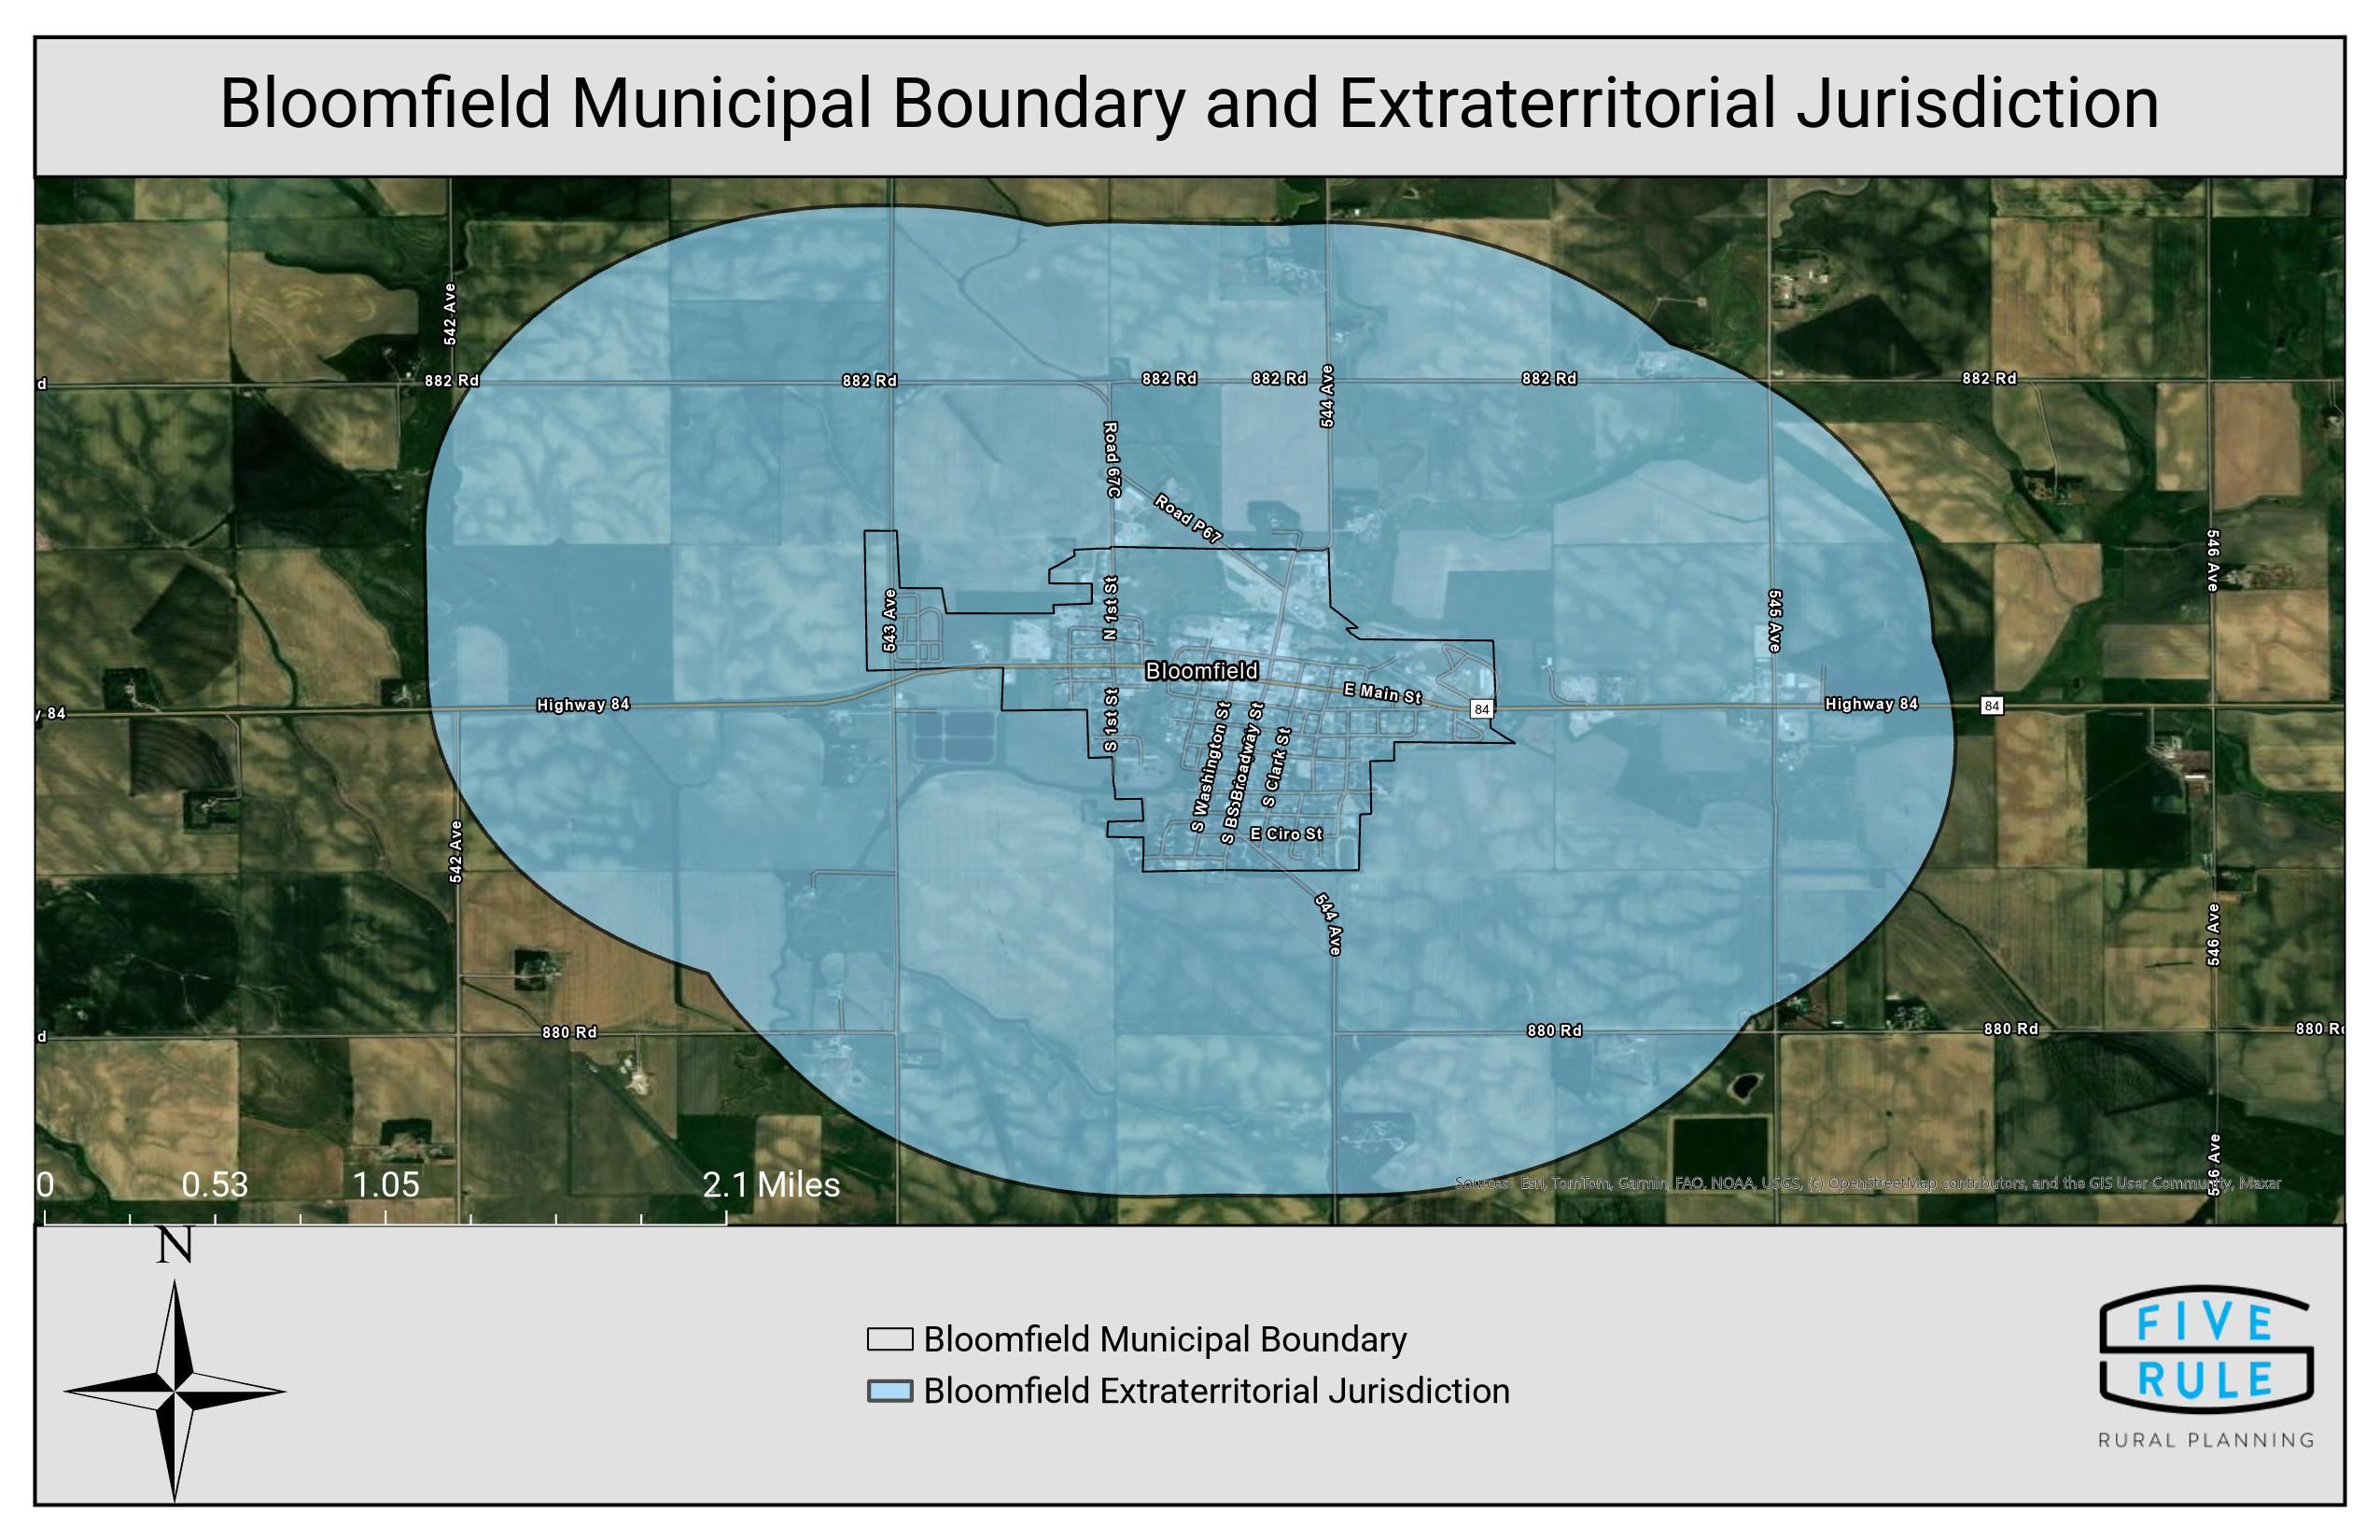
\includepdf[angle=90]{maps/boundary_etj.pdf}
\end{landscape}
\pagebreak